\documentclass[border=1pt]{standalone}
\usepackage{tikz}
\usetikzlibrary{calc}

\begin{document}
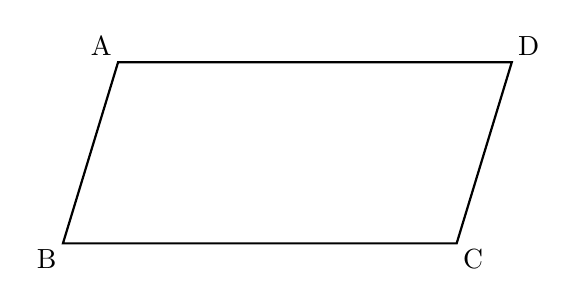
\begin{tikzpicture}
    \pgfmathsetmacro{\X}{5}
    \pgfmathsetmacro{\d}{0.14*\X}
    \pgfmathsetmacro{\Y}{0.46*\X}
    \coordinate (B) at (0,0);
    \coordinate (C) at (\X,0);
    \coordinate (A) at (\d,\Y);
    \coordinate (D) at ($(C)+(A)-(B)$);
    \draw [thick] (A)--(B)--(C)--(D)--cycle;
    \node[below left, outer sep=-1pt] at (B) {B};
    \node[below right, outer sep=-1pt] at (C) {C};
    \node[above right, outer sep=-1pt] at (D) {D};
    \node[above left, outer sep=-1pt] at (A) {A};
\end{tikzpicture}
\end{document}
